\documentclass{article}
\usepackage[utf8]{inputenc}
\usepackage[spanish]{babel}
\usepackage{graphicx}
\usepackage{longtable}
\usepackage{float}
\graphicspath{{./img/}}

\title{Práctica 1. Análisis de eficiencia de algoritmos}
\author{Noelia Escalera Mejías \\
		\and Alejandro Menor Molinero \\
		\and Javier Núñez Suárez \\
		\and Adra Sánchez Ruiz \\
		\and Jesús Torres Sánchez}
\begin{document}
	\maketitle
	\tableofcontents
	\section{Introducción}
	El objetivo de esta práctica será analizar la eficiencia de distintos algoritmos de distintos órdenes de eficiencia ($n*log(n)$,$n^2$,$n^3$ y $(\frac{1+\sqrt{5}}{2})^n$). Vamos a calcular su eficiencia empírica e híbrida y comprobaremos su eficiencia en distintas condiciones.
	\section{Eficiencia empírica}
	Vamos a medir el tiempo que tarda en ejecutarse cada uno de los ocho algoritmos: Quicksort, Mergesort, Heapsort, Inserción, Selección, Burbuja, Floyd y Fibonacci.
	
	\
	Además, los compararemos entre ellos cuando sea interesante hacerlo.
	\subsection{Algoritmos de ordenación}
	\subsubsection{Ordenación rápida}
	Empezamos con los algoritmos de ordenación rápidos. Estos pertenecen al orden de eficiencia $O(n*log(n))$ es decir, "superlineales".
	
	\
	He aquí una tabla comparativa del tiempo que tarda cada algoritmo según el tamaño del vector a ordenar.
		\begin{longtable}{|c|c|c|c|}
			\hline
			Tamaño del vector & Tiempo con Quicksort & Tiempo con Mergesort & Tiempo con Heapsort \\ \hline
			500	     &  0.000125572	 &  0.000185121	 &  0.000192113  \\ \hline
			1000	 &  0.000271314	 &  0.000389135	 &  0.000444516  \\ \hline
			1500	 &  0.00041891	 &  0.000760708	 &  0.000705254  \\ \hline
			2000	 &  0.000594146	 &  0.00102568	 &  0.00097424  \\ \hline
			2500	 &  0.000740502	 &  0.000482617	 &  0.000443686  \\ \hline
			3000	 &  0.000596825	 &  0.000494674	 &  0.000381796  \\ \hline
			3500	 &  0.000343663	 &  0.000452999	 &  0.000429375  \\ \hline
			4000	 &  0.000373585	 &  0.000644118	 &  0.00053697  \\ \hline
			4500	 &  0.00042863	 &  0.000694048	 &  0.000605903  \\ \hline
			5000	 &  0.000513286	 &  0.000788472	 &  0.000634107  \\ \hline
			5500	 &  0.000557894	 &  0.000948842	 &  0.000715611  \\ \hline
			6000	 &  0.000605284	 &  0.00105457	 &  0.000794382  \\ \hline
			6500	 &  0.000657624	 &  0.000926247	 &  0.000862167  \\ \hline
			7000	 &  0.000714435	 &  0.00100227	 &  0.000929307  \\ \hline
			7500	 &  0.000757684	 &  0.0011178	 &  0.00100083  \\ \hline
			8000	 &  0.000831217	 &  0.00123515	 &  0.00108477  \\ \hline
			8500	 &  0.00087632	 &  0.00131409	 &  0.00114999  \\ \hline
			9000	 &  0.000951436	 &  0.00139895	 &  0.00124178  \\ \hline
			9500	 &  0.00100672	 &  0.00153253	 &  0.001302  \\ \hline
			10000	 &  0.00104054	 &  0.00163203	 &  0.00136841  \\ \hline
			10500	 &  0.00111741	 &  0.00176789	 &  0.00144557  \\ \hline
			11000	 &  0.0011769	 &  0.00188453	 &  0.00152554  \\ \hline
			11500	 &  0.00124374	 &  0.00208893	 &  0.00161126  \\ \hline
			12000	 &  0.00128353	 &  0.00217296	 &  0.00168296  \\ \hline
			12500	 &  0.00134991	 &  0.00229752	 &  0.0017724  \\ \hline
			13000	 &  0.00142095	 &  0.00192418	 &  0.00186281  \\ \hline
			13500	 &  0.00144951	 &  0.00202339	 &  0.00193143  \\ \hline
			14000	 &  0.00152673	 &  0.00208988	 &  0.00199139  \\ \hline
			14500	 &  0.00158276	 &  0.00219523	 &  0.00207509  \\ \hline
			15000	 &  0.0016307	 &  0.00232089	 &  0.00216104  \\ \hline
			15500	 &  0.0016855	 &  0.0024091	 &  0.00223611  \\ \hline
			16000	 &  0.00175315	 &  0.00251567	 &  0.00231843  \\ \hline
			16500	 &  0.00180967	 &  0.00262037	 &  0.00240901  \\ \hline
			17000	 &  0.00187919	 &  0.0027362	 &  0.00250793  \\ \hline
			17500	 &  0.00192917	 &  0.00287752	 &  0.00256264  \\ \hline
			18000	 &  0.0020248	 &  0.00300007	 &  0.00263882  \\ \hline
			18500	 &  0.00204495	 &  0.00310153	 &  0.00272534  \\ \hline
			19000	 &  0.00211357	 &  0.00325465	 &  0.00280503  \\ \hline
			19500	 &  0.00218022	 &  0.00338002	 &  0.00289392  \\ \hline
			20000	 &  0.00223461	 &  0.00350399	 &  0.00304415  \\ \hline
			20500	 &  0.00232654	 &  0.00358945	 &  0.00314781  \\ \hline
			21000	 &  0.0023512	 &  0.00372468	 &  0.00322618  \\ \hline
			21500	 &  0.0024141	 &  0.00385273	 &  0.00330935  \\ \hline
			22000	 &  0.00248485	 &  0.00398946	 &  0.00339943  \\ \hline
			22500	 &  0.00255673	 &  0.00411845	 &  0.00348261  \\ \hline
			23000	 &  0.00264539	 &  0.00433311	 &  0.00357741  \\ \hline
			23500	 &  0.00272772	 &  0.00445179	 &  0.00366066  \\ \hline
			24000	 &  0.00270691	 &  0.00454967	 &  0.00373309  \\ \hline
			24500	 &  0.00285553	 &  0.00466454	 &  0.00382896  \\ \hline
			25000	 &  0.00282962	 &  0.0048426	 &  0.00392208  \\ \hline
		\end{longtable}
		\begin{center}
		\end{center}
		\begin{figure}[H]
		\centering
		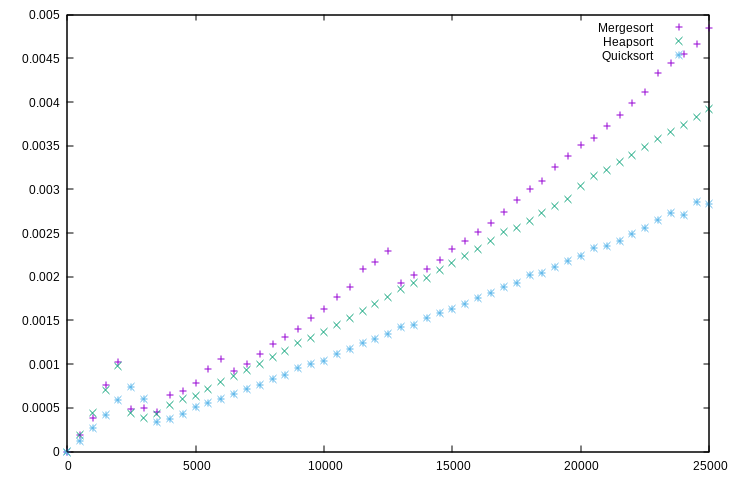
\includegraphics[totalheight=8cm]{img/ordenacion_rapida}
		\caption{Comparación gráfica del rendimiento de los algoritmos de ordenación rápida}
		\label{fig:ordenacion_rapida}
		\end{figure}
		\
		Podemos apreciar que el más rápido de estos tres algoritmos sería Quicksort, seguido por Heapsort y por último, Mergesort. Vamos a concretar estos datos:
		\
		\begin{longtable}{|c||c|}
			\hline
			Tiempos Heapsort/Tiempos Quicksort & Tiempos Mergesort/Tiempos Heapsort \\ \hline
			1.52990316312554	&  0.963604753452395  \\ \hline
			1.63838209602158	&  0.875412808537825  \\ \hline
			1.68354539161156	&  1.07862982698432  \\ \hline
			1.63973164845004	&  1.05280013138446  \\ \hline
			0.599169212237104	&  1.0877444859653  \\ \hline
			0.639711808319021	&  1.29565003300192  \\ \hline
			1.24940712267541	&  1.05501950509461  \\ \hline
			1.43734357642839	&  1.1995418738477  \\ \hline
			1.41358047733476	&  1.145477081315  \\ \hline
			1.23538728895781	&  1.24343683321585  \\ \hline
			1.28270065639709	&  1.32591869046172  \\ \hline
			1.31241202476854	&  1.32753511534753  \\ \hline
			1.31103335644685	&  1.07432434783516  \\ \hline
			1.30075794159021	&  1.07851334381426  \\ \hline
			1.32090686882658	&  1.11687299541381  \\ \hline
			1.30503827520371	&  1.13862846502023  \\ \hline
			1.31229459558152	&  1.14269689301646  \\ \hline
			1.30516398370463	&  1.12656831322779  \\ \hline
			1.29330896376351	&  1.17705837173579  \\ \hline
			1.31509600784208	&  1.19264694060991  \\ \hline
			1.29367913299505	&  1.22297086962236  \\ \hline
			1.29623587390602	&  1.23531995227919  \\ \hline
			1.29549584318266	&  1.29645743083053  \\ \hline
			1.31119646599612	&  1.29115368160859  \\ \hline
			1.31297642065027	&  1.29627623561273  \\ \hline
			1.31096097681129	&  1.03294485213199  \\ \hline
			1.33247097294948	&  1.04761239081924  \\ \hline
			1.30434981954897	&  1.0494579163298  \\ \hline
			1.31105789886022	&  1.0578962840166  \\ \hline
			1.32522229717299	&  1.07396901491874  \\ \hline
			1.32667457727677	&  1.0773620260184  \\ \hline
			1.32243675669509	&  1.08507481355918  \\ \hline
			1.33118745406621	&  1.08773728627112  \\ \hline
			1.33458032450151	&  1.0910192868222  \\ \hline
			1.32836401146607	&  1.12287328692286  \\ \hline
			1.30324970367444	&  1.13689831060853  \\ \hline
			1.33271718134918	&  1.13803415353681  \\ \hline
			1.32715263748066	&  1.16029062077767  \\ \hline
			1.32735228554916	&  1.16797285343064  \\ \hline
			1.36227350633891	&  1.1510569452885  \\ \hline
			1.3530005931555	    &  1.14030071700643  \\ \hline
			1.3721418849949	    &  1.15451710691902  \\ \hline
			1.37084213578559	&  1.16419538580084  \\ \hline
			1.3680624584985	    &  1.17356733334706  \\ \hline
			1.3621344451702	    &  1.18257571189424  \\ \hline
			1.35231856172436	&  1.21124221154411  \\ \hline
			1.34202190840702	&  1.21611676582911  \\ \hline
			1.37909646053988	&  1.21874104294298  \\ \hline
			1.34089293406128	&  1.21822635911579  \\ \hline
			1.38608010969671	&  1.23470199485987  \\ \hline
		\end{longtable}
	Podemos ver que Heapsort es aproximadamente 1.3 veces más lento que Quicksort y que Mergesort es aproximadamente 1.2 veces más lento que Heapsort.
	\subsubsection{Ordenación lentos}
		Estos algoritmos de ordenación, menos sofisticados, son de orden $O(n ^2)$ es decir, cuadráticos.
		\begin{longtable}{|c|c|c|c|}
			\hline
			Tamaño del vector & Tiempo con Burbuja & Tiempo con Selección & Tiempo con Inserción \\ \hline
			500	   &    0.00178596	&  0.00147628  	   &  0.00114028   \\ \hline
			1000  &	    0.0028655	&  0.0022588  	   &  0.00172961   \\ \hline
			1500  &	    0.00448784	&  0.00309903  	   &  0.00230721   \\ \hline
			2000  &	    0.00786624	&  0.00525987  	   &  0.00405115   \\ \hline
			2500  &	    0.0124692	&  0.00811555  	   &  0.00630397   \\ \hline
			3000  &	    0.0181514	&  0.0116717  	   &  0.00910679   \\ \hline
			3500  &	    0.0252785	&  0.0157854  	   &  0.0125022   \\ \hline
			4000  &	    0.0337448	&  0.0205625  	   &  0.0158871   \\ \hline
			4500  &	    0.0436306	&  0.0268227  	   &  0.0201791   \\ \hline
			5000  &	    0.0551609	&  0.0331552  	   &  0.026194   \\ \hline
			5500  &	    0.0681233	&  0.0401148  	   &  0.030802   \\ \hline
			6000  &	    0.0824843	&  0.0467118  	   &  0.035932   \\ \hline
			6500  &	    0.0984357	&  0.0540054   	   &  0.042335   \\ \hline
			7000  &	    0.11589	    &  0.0626111   	   &  0.0497211   \\ \hline
			7500  &	    0.135017	&  0.0717969   	   &  0.0573054   \\ \hline
			8000  &	    0.155683	&  0.0817153   	   &  0.0657382   \\ \hline
			8500  &	    0.176902	&  0.0921947   	   &  0.0768291   \\ \hline
			9000  &	    0.199919	&  0.103297	       &  0.0861508   \\ \hline
			9500  &	    0.225075	&  0.115035	       &  0.0981397   \\ \hline
			10000  &	0.251881	&  0.127486	       &  0.103923   \\ \hline
			10500  &	0.279234	&  0.140492	       &  0.122772   \\ \hline
			11000  &	0.309941	&  0.154166	       &  0.131101   \\ \hline
			11500  &	0.34121	    &  0.171219	       &  0.142071   \\ \hline
			12000  &	0.371406	&  0.183355	       &  0.158711   \\ \hline
			12500  &	0.405278	&  0.198969	       &  0.168258   \\ \hline
			13000  &	0.441736	&  0.215243	       &  0.178126   \\ \hline
			13500  &	0.478529	&  0.232051	       &  0.195711   \\ \hline
			14000  &	0.517851	&  0.249406	       &  0.215179   \\ \hline
			14500  &	0.557069	&  0.26754	       &  0.223471   \\ \hline
			15000  &	0.623507	&  0.286271	       &  0.245298   \\ \hline
			15500  &	0.64346	    &  0.305662	       &  0.257939   \\ \hline
			16000  &	0.693738	&  0.325702	       &  0.277471   \\ \hline
			16500  &	0.734539	&  0.346204	       &  0.297803   \\ \hline
			17000  &	0.778796	&  0.367458	       &  0.311583   \\ \hline
			17500  &	0.829418	&  0.39475	       &  0.322414   \\ \hline
			18000  &	0.880487	&  0.412826	       &  0.352076   \\ \hline
			18500  &	0.933294	&  0.435126	       &  0.360694   \\ \hline
			19000  &	0.986121	&  0.460939	       &  0.379935   \\ \hline
			19500  &	1.07066	    &  0.483263	       &  0.396013   \\ \hline
			20000  &	1.09964	    &  0.515923	       &  0.421674   \\ \hline
			20500  &	1.15639	    &  0.544332	       &  0.447574   \\ \hline
			21000  &	1.22045	    &  0.5604	       &  0.471736   \\ \hline
			21500  &	1.32645	    &  0.590167	       &  0.483069   \\ \hline
			22000  &	1.39171	    &  0.618805	       &  0.504104   \\ \hline
			22500  &	1.55601	    &  0.646724	       &  0.53811   \\ \hline
			23000  &	1.52041	    &  0.671924	       &  0.56646   \\ \hline
			23500  &	1.60414	    &  0.701547	       &  0.596336   \\ \hline
			24000  &	1.6872	    &  0.745452	       &  0.613182   \\ \hline
			24500  &	1.7148	    &  0.770377	       &  0.635088   \\ \hline
			25000  &	1.78348	    &  0.79409	       &  0.638414   \\ \hline
		\end{longtable}
	\begin{figure}[H]
		\centering
		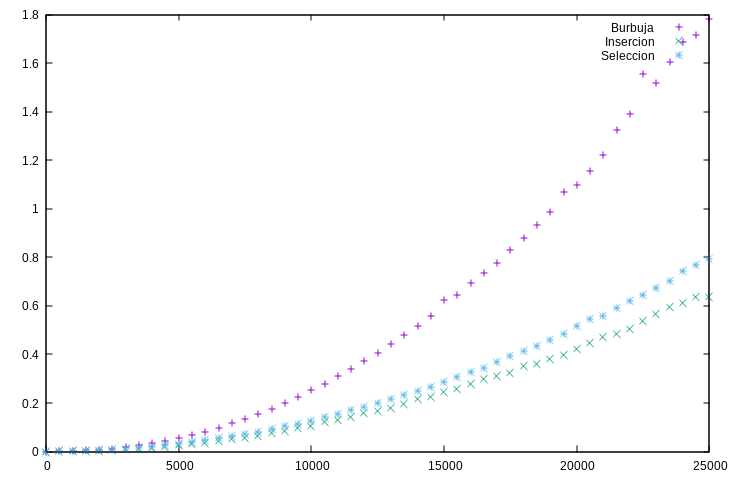
\includegraphics[totalheight=8cm]{img/ordenacion_lenta}
		\caption{Comparación gráfica del rendimiento de los algoritmos de ordenación lenta}
		\label{fig:ordenacion_lenta}
	\end{figure}
Aquí vemos que el más lento es con diferencia Burbuja, seguido de Seleción y finalmente de Inserción. Volvemos a concretar estas diferencias con una tabla:
\begin{longtable}{|c||c|}
	\hline
	Tiempos Burbuja/Tiempos Selección & Tiempos Selección/Tiempos Inserción \\ \hline
	1.20977050424039	&  1.29466446837619 \\ \hline
	1.26859394368691	&  1.3059591468597 \\ \hline
	1.448143451338	    &  1.34319372748905 \\ \hline
	1.49551985125108	&  1.29836466188613 \\ \hline
	1.53645778782707	&  1.28737129142429 \\ \hline
	1.55516334381453	&  1.28164808895341 \\ \hline
	1.60138482395125	&  1.2626097806786 \\ \hline
	1.64108449848024	&  1.29428907730171 \\ \hline
	1.62662968306695	&  1.32923172985911 \\ \hline
	1.66371790850304	&  1.2657555165305 \\ \hline
	1.69820864119976	&  1.30234400363613 \\ \hline
	1.76581292093218	&  1.30000556606924 \\ \hline
	1.82270106322701	&  1.27566788709106 \\ \hline
	1.85094975172134	&  1.25924607460414 \\ \hline
	1.88054080329374	&  1.25288192735763 \\ \hline
	1.90518789015031	&  1.24304133669617 \\ \hline
	1.91878708862874	&  1.19999713650166 \\ \hline
	1.93538050475812	&  1.1990254298277 \\ \hline
	1.95657843265093	&  1.17215561082824 \\ \hline
	1.97575420046123	&  1.22673517893055 \\ \hline
	1.9875437747345	    &  1.1443325839768 \\ \hline
	2.01043680188887	&  1.1759330592444 \\ \hline
	1.99282789877292	&  1.20516502312224 \\ \hline
	2.02561151863871	&  1.15527594180618 \\ \hline
	2.03689016882027	&  1.18252326783868 \\ \hline
	2.05226650808621	&  1.20837497052648 \\ \hline
	2.06217167777773	&  1.18568194940499 \\ \hline
	2.0763373776092	    &  1.15906291970871 \\ \hline
	2.08218957912835	&  1.19720232155403 \\ \hline
	2.17803060736156	&  1.16703356733443 \\ \hline
	2.1051357381683	    &  1.18501661245488 \\ \hline
	2.12997770968554	&  1.17382357075154 \\ \hline
	2.12169414564823	&  1.16252690537033 \\ \hline
	2.1194150079737	    &  1.17932621484484 \\ \hline
	2.10112222925902	&  1.22435750308609 \\ \hline
	2.13282835867896	&  1.17254797259683 \\ \hline
	2.14488217206051	&  1.20635774368301 \\ \hline
	2.13937419051111	&  1.21320489031018 \\ \hline
	2.21548101137476	&  1.22032105006654 \\ \hline
	2.13140332956662	&  1.22351152786276 \\ \hline
	2.12442039049698	&  1.21618324567558 \\ \hline
	2.17781941470378	&  1.18795258364848 \\ \hline
	2.24758415838229	&  1.2217033177455 \\ \hline
	2.24902836919547	&  1.22753439766397 \\ \hline
	2.40598771655297	&  1.20184348924941 \\ \hline
	2.26277078955358	&  1.18618084242488 \\ \hline
	2.28657524014785	&  1.17642906012718 \\ \hline
	2.26332480159688	&  1.21571083299901 \\ \hline
	2.22592315191134	&  1.21302402186784 \\ \hline
	2.24594189575489	&  1.243848035914 \\ \hline
\end{longtable}
Aquí vemos que Burbuja es aproximadamente 2 veces más lento que Selección y que éste es aproximadamente 1.2 veces más lento que inserción.

\

Por último, en las figuras \ref{fig:ordenacion} y \ref{fig:ordenacion_zoom}, se muestra el rendimiento de todos los algoritmos de ordenación, rápidos y lentos.
	\begin{figure}[H]
		\centering
		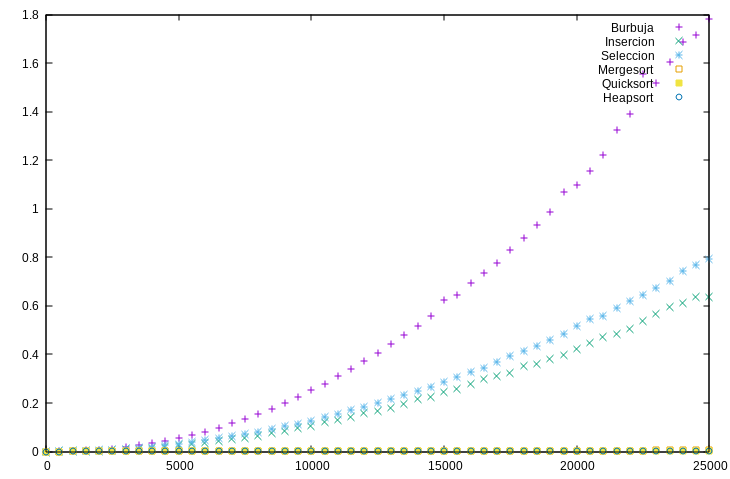
\includegraphics[totalheight=8cm]{img/ordenacion}
		\caption{Comparación gráfica del rendimiento de los algoritmos de ordenación}
		\label{fig:ordenacion}
	\end{figure}
	\begin{figure}[H]
		\centering
		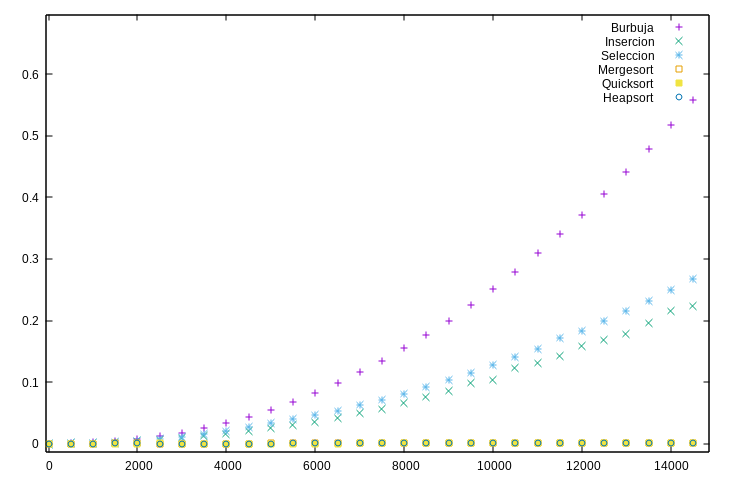
\includegraphics[totalheight=8cm]{img/ordenacion_zoom}
		\caption{\textit{Zoom} en el intervalo [0-15000] de la figura \ref{fig:ordenacion}}
		\label{fig:ordenacion_zoom}
	\end{figure}
Se puede apreciar claramente la gran diferencia entre los algoritmos $O(n*log(n))$ y $O(n^2)$.
\subsection{Floyd}
Dado un conjunto de nodos de un grafo dirigido, el algoritmo de Floyd calcula el costo del camino mínimo entre cada par. Pertenece al orden de eficiencia $O(n ^3)$, se muestra una gráfica en la figura \ref{fig:floyd}.
\begin{longtable}{|c||c|}
	\hline
	Tamaño & Tiempo  \\ \hline
	1       & 1.954e-07    \\ \hline
	21      & 0.000155079 \\ \hline
	41      & 0.00103966 \\ \hline
	61      & 0.00231581 \\ \hline
	81      & 0.00315898 \\ \hline
	101     & 0.00603818 \\ \hline
	121     & 0.0102868 \\ \hline
	141     & 0.0163929 \\ \hline
	161     & 0.0241221 \\ \hline
	181     & 0.0351787 \\ \hline
	201     & 0.0473705 \\ \hline
	221     & 0.0620468 \\ \hline
	241     & 0.0834537 \\ \hline
	261     & 0.103527 \\ \hline
	281     & 0.128019 \\ \hline
	301     & 0.1575 \\ \hline
	321     & 0.194009 \\ \hline
	341     & 0.231567 \\ \hline
	361     & 0.275895 \\ \hline
	381     & 0.32918 \\ \hline
	401     & 0.367902 \\ \hline
	421     & 0.4349 \\ \hline
	441     & 0.490013 \\ \hline
	461     & 0.562313 \\ \hline
	481     & 0.631398 \\ \hline
	501     & 0.716334 \\ \hline
	521     & 0.832386 \\ \hline
	541     & 0.918103 \\ \hline
	561     & 1.03886 \\ \hline
	581     & 1.12256 \\ \hline
	601     & 1.23978 \\ \hline
	621     & 1.36486 \\ \hline
	641     & 1.5045 \\ \hline
	661     & 1.64389 \\ \hline
	681     & 1.79002 \\ \hline
	701     & 1.96247 \\ \hline
	721     & 2.16406 \\ \hline
	741     & 2.39603 \\ \hline
	761     & 2.64711 \\ \hline
	781     & 2.81278 \\ \hline
	801     & 3.1552 \\ \hline
	821     & 3.19514 \\ \hline
	841     & 3.45967 \\ \hline
	861     & 3.82836 \\ \hline
	881     & 3.88608 \\ \hline
	901     & 4.45056 \\ \hline
	921     & 4.35145 \\ \hline
	941     & 4.50856 \\ \hline
	961     & 4.88424 \\ \hline
	981     & 5.52174 \\ \hline
	1001    & 5.60464 \\ \hline
\end{longtable}
\begin{figure}[H]
	\centering
	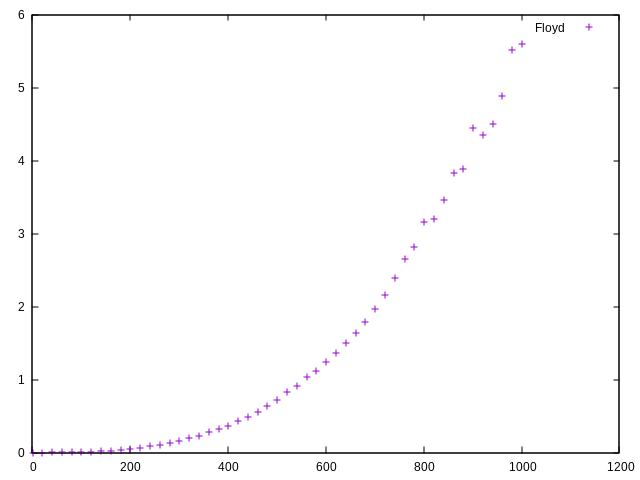
\includegraphics[totalheight=8cm]{img/floyd}
	\caption{Tiempos de ejecución en el algoritmo de Floyd}
	\label{fig:floyd}
\end{figure}
\subsection{Fibonacci}
Este algoritmo calcula los números de la sucesión de Fibonacci. 
\

Hace uso de la recursión y como hemos visto en clase, esto puede derivar muy facilmente en un algoritmo de orden exponencial, es este uno de esos casos.
\

$fib(n) \in O((\frac{1+\sqrt5}{2})^n)$

\begin{longtable}{|c||c|}
	\hline
	Tamaño & Tiempo  \\ \hline
	0   & 2.856e-07  \\ \hline
	1   & 1.512e-07  \\ \hline
	2   & 2.096e-07  \\ \hline
	3   & 2.086e-07  \\ \hline
	4   & 2.698e-07  \\ \hline
	5   & 3.788e-07  \\ \hline
	6   & 5.074e-07  \\ \hline
	7   & 7.382e-07  \\ \hline
	8   & 1.0928e-06  \\ \hline
	9   & 1.599e-06  \\ \hline
	10  &  2.4596e-06  \\ \hline
	11  &  3.8526e-06  \\ \hline
	12  &  6.078e-06  \\ \hline
	13  &  9.6922e-06  \\ \hline
	14  &  1.44386e-05  \\ \hline
	15  &  2.0433e-05  \\ \hline
	16  &  3.66042e-05  \\ \hline
	17  &  4.68404e-05  \\ \hline
	18  &  7.15016e-05  \\ \hline
	19  &  0.000113647  \\ \hline
	20  &  0.000181842  \\ \hline
	21  &  0.000291334  \\ \hline
	22  &  0.000485881  \\ \hline
	23  &  0.000766585  \\ \hline
	24  &  0.00061927  \\ \hline
	25  &  0.000491851  \\ \hline
	26  &  0.000754886  \\ \hline
	27  &  0.0013577  \\ \hline
	28  &  0.00209638  \\ \hline
	29  &  0.00339488  \\ \hline
	30  &  0.00540311  \\ \hline
	31  &  0.00876756  \\ \hline
	32  &  0.0143048  \\ \hline
	33  &  0.0226266  \\ \hline
	34  &  0.036777  \\ \hline
	35  &  0.0581737  \\ \hline
	36  &  0.0948025  \\ \hline
	37  &  0.158607  \\ \hline
	38  &  0.260101  \\ \hline
	39  &  0.40173  \\ \hline
	40  &  0.654265  \\ \hline
	41  &  1.06958  \\ \hline
	42  &  1.70722  \\ \hline
	43  &  2.74853  \\ \hline
	44  &  4.60926  \\ \hline
	45  &  7.51057  \\ \hline
	46  &  11.6822  \\ \hline
	47  &  18.6488  \\ \hline
	48  &  30.9733  \\ \hline
	49  &  52.57  \\ \hline
	50  &  83.3349  \\ \hline
\end{longtable}

\begin{figure}[H]
	\centering
	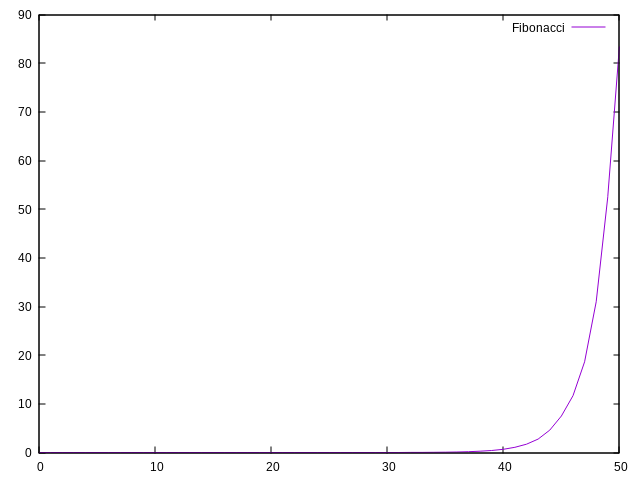
\includegraphics[totalheight=8cm]{img/fibonacci}
	\caption{Tiempos de ejecución en el algoritmo de Fibonacci}
	\label{fig:fibonacci}
\end{figure}


	\section{Eficiencia híbrida}
	Ajuste de las diferentes funciones de acuerdo a la eficiencia teórica de los algoritmos y los datos obtenidos en la eficiencia empírica.
	
	\subsection{Algoritmos de ordenación rápidos}
	
	
	Para el algoritmo Mergesort:

	\begin{longtable}{|c|c|c|}
		\hline
	 	Constante		& Valor			& Error estándar	\\ \hline
		a0              & 3.66473e-12	& 12.16 \\ \hline
		a1              & 8.67345e-08	& 13.28 \\ \hline
		a2              & 0.000308646	& 20.18 \\ \hline
	\end{longtable}

	\begin{figure}[H]
		\centering
		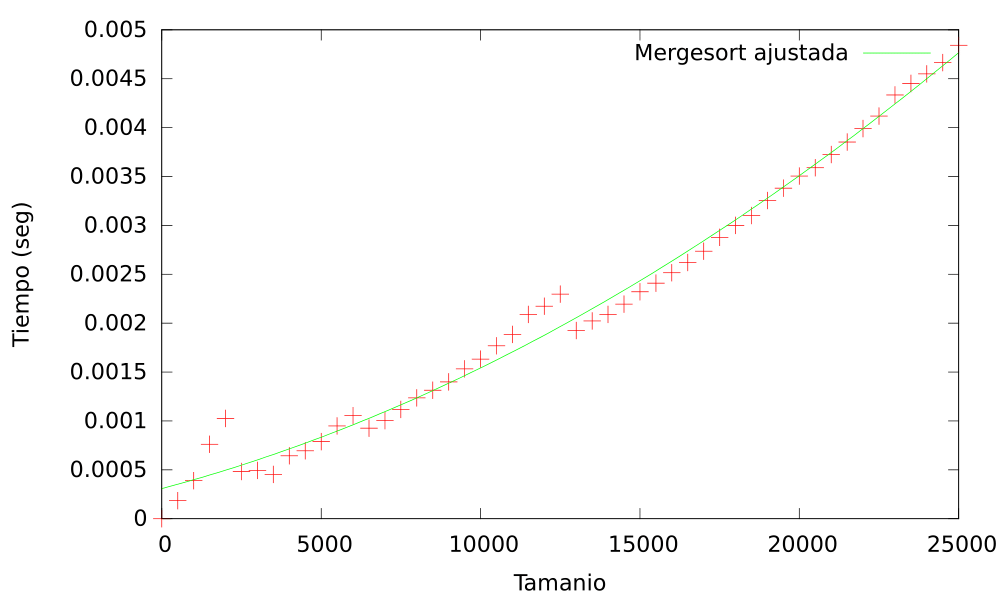
\includegraphics[totalheight=8cm]{img/Mergesort_ajustada}
		\caption{Ajuste función Mergesort}
		\label{fig:Mergesort_ajustada}
	\end{figure}

	Para el algoritmo Heapsort:

	\begin{longtable}{|c|c|c|}
		\hline
		Constante		& Valor			& Error estándar	\\ \hline
		a0              & 2.32227e-12	& 14.09 \\ \hline
		a1              & 9.24005e-08	& 9.152 \\ \hline
		a2              & 0.000224702	& 20.34 \\ \hline
	\end{longtable}

	\begin{figure}[H]
		\centering
		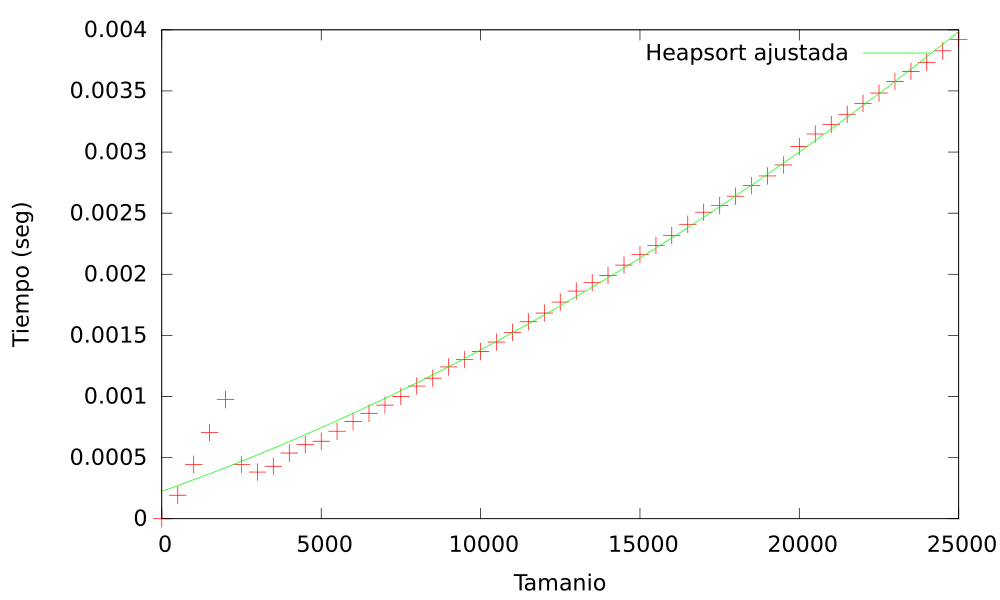
\includegraphics[totalheight=8cm]{img/Heapsort_ajustada}
		\caption{Ajuste función Heapsort}
		\label{fig:Heapsort_ajustada}
	\end{figure}

	Para el algoritmo Quicksort:

	\begin{longtable}{|c|c|c|}
		\hline
		Constante		& Valor			& Error estándar	\\ \hline
		a0              & 1.37793e-12	& 18.84 \\ \hline
		a1              & 7.47827e-08	& 8.974 \\ \hline
		a2              & 0.000181972	& 19.93 \\ \hline
	\end{longtable}
	
	

	\begin{figure}[H]
		\centering
		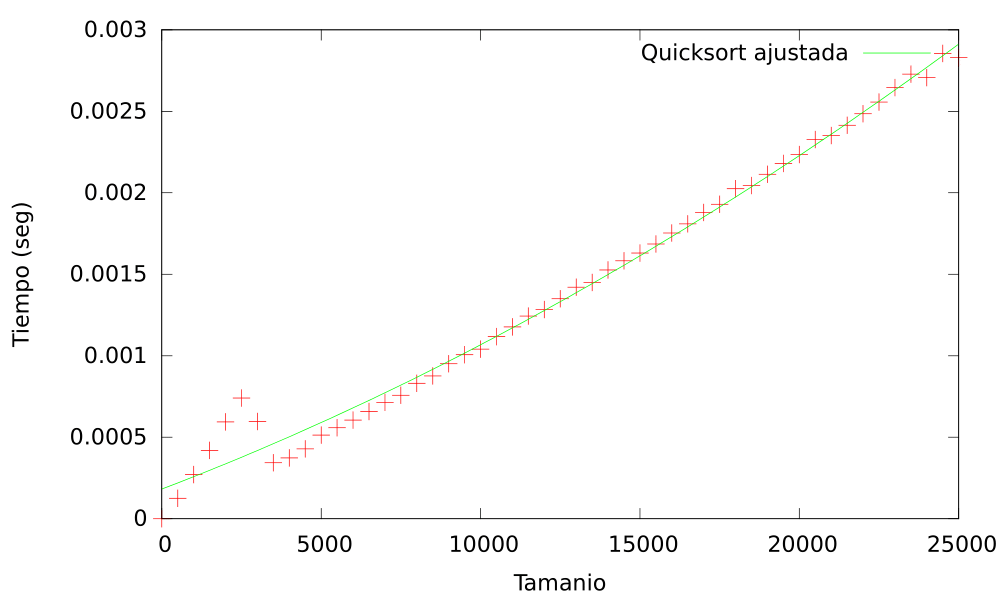
\includegraphics[totalheight=8cm]{img/Quicksort_ajustada}
		\caption{Ajuste función Quicksort}
		\label{fig:Quicksort_ajustada}
	\end{figure}
	
	
	\begin{figure}[H]
		\centering
		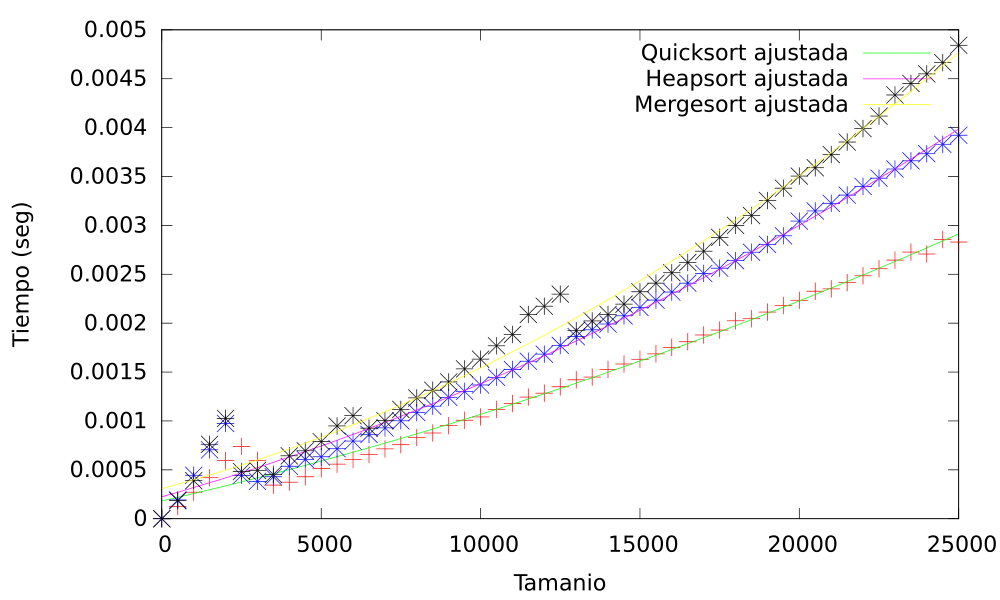
\includegraphics[totalheight=8cm]{img/AlgOrdenacionRapidos_ajustados}
		\caption{Comparativa ajuste para algoritmos de ordenación rápidos}
		\label{fig:AlgOrdenacionRapidos_ajustados}
	\end{figure}

	\
	
	Podemos ver que los tiempos se ajustan bastante bien a sus respectivas curvas teóricas (quizá Mergesort sea el que menos se ajusta, aunque no hay un error muy grande) excepto al principio con los tamaños más pequeños.

	\subsection{Algoritmos de ordenación lentos}


Para el algoritmo Burbuja:

	\begin{longtable}{|c|c|c|}
		\hline
		Constante		& Valor			& Error estándar	\\ \hline
		a0              & 3.25024e-09	& 1.809 \\ \hline
		a1              & -9.48063e-06	& 16.03 \\ \hline
		a2              & 0.0160101		& 51.32 \\ \hline
	\end{longtable}

	\begin{figure}[H]
		\centering
		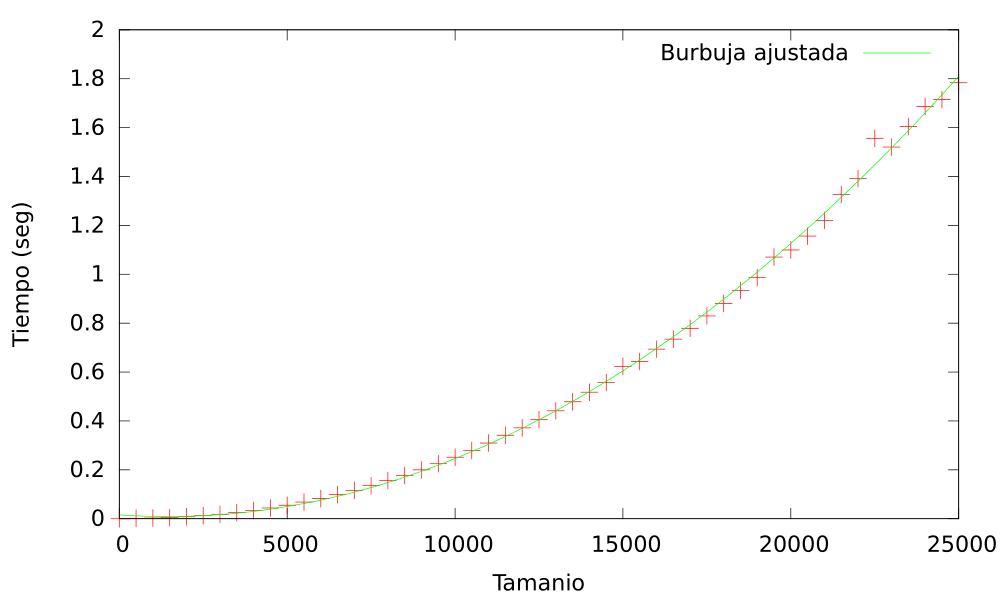
\includegraphics[totalheight=8cm]{img/Burbuja_ajustada}
		\caption{Ajuste función Burbuja}
		\label{fig:Burbuja_ajustada}
	\end{figure}

Para el algoritmo Insercion:

	\begin{longtable}{|c|c|c|}
		\hline
		Constante		& Valor			& Error estándar	\\ \hline
		a0              & 1.02502e-09	& 1.459 \\ \hline
		a1              & 8.53837e-07	& 45.29 \\ \hline
		a2              & -0.00285116	& 73.31 \\ \hline
	\end{longtable}

	\begin{figure}[H]
		\centering
		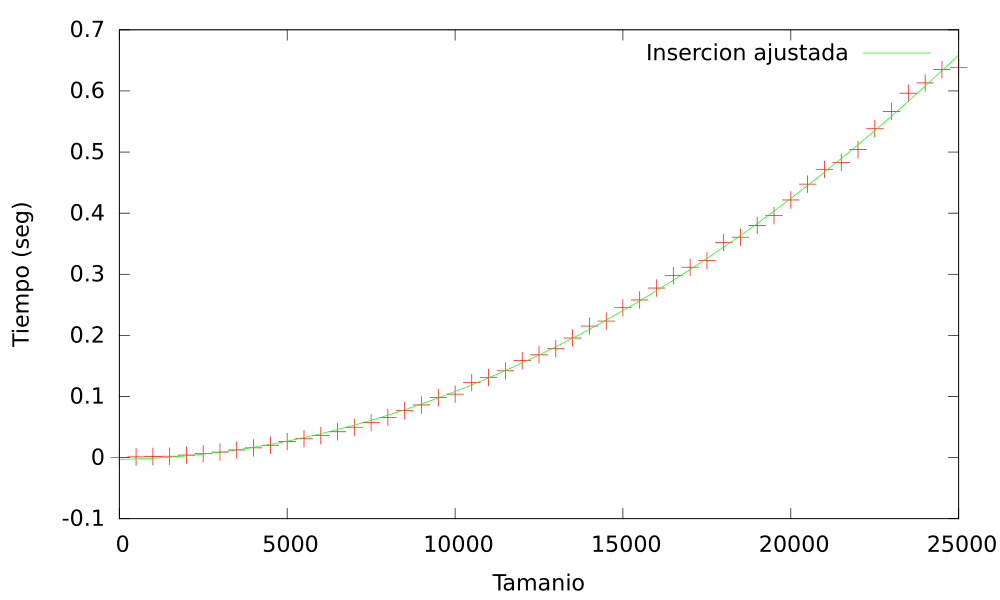
\includegraphics[totalheight=8cm]{img/Insercion_ajustada}
		\caption{Ajuste función Inserción}
		\label{fig:Insercion_ajustada}
	\end{figure}

	Para el algoritmo de Seleccion:

	\begin{longtable}{|c|c|c|}
		\hline
		Constante		& Valor			& Error estándar	\\ \hline
		a0              & 1.28478e-09	& 0.5517 \\ \hline
		a1              & -1.91843e-07	& 95.52 \\ \hline
		a2              & 0.00095162	& 104.1 \\ \hline
	\end{longtable}

	\begin{figure}[H]
		\centering
		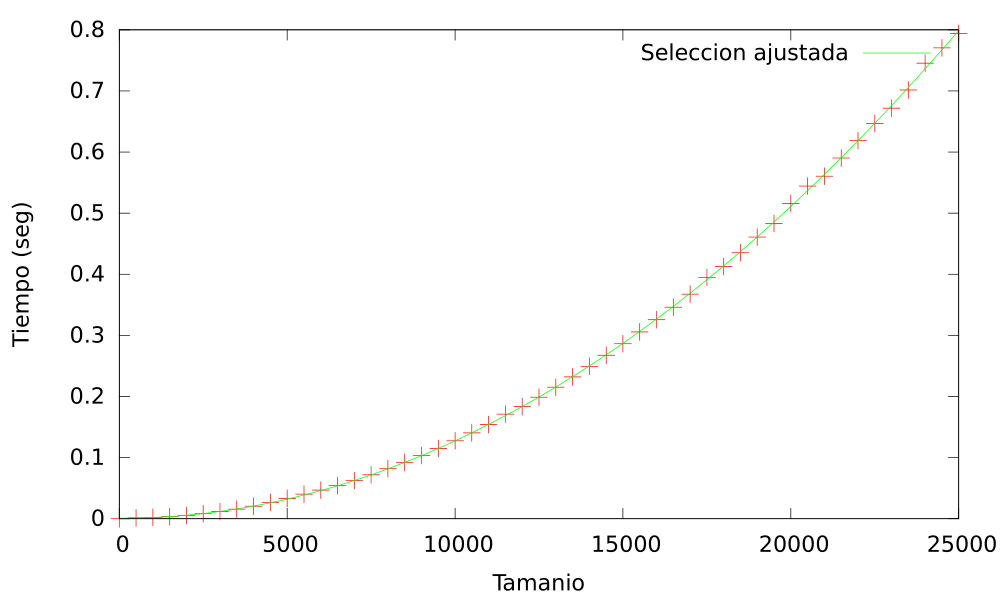
\includegraphics[totalheight=8cm]{img/Seleccion_ajustada}
		\caption{Ajuste función Selección}
		\label{fig:Seleccion_ajustada}
	\end{figure}
	
	\begin{figure}[H]
		\centering
		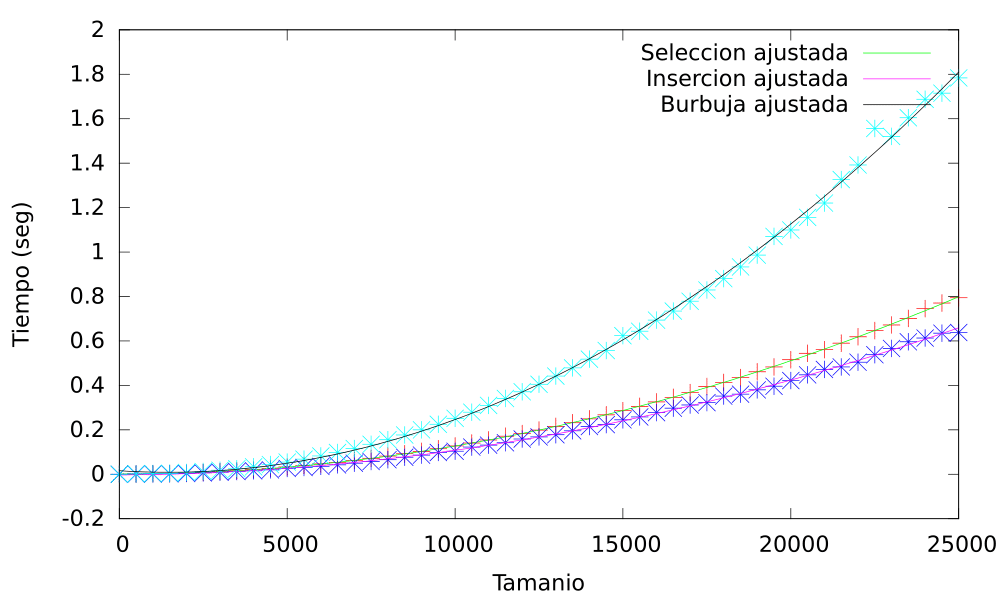
\includegraphics[totalheight=8cm]{img/AlgOrdenacionLentos_ajustados}
		\caption{Comparativa ajuste para algoritmos de ordenación lentos}
		\label{fig:AlgOrdenacionLentos_ajustados}
	\end{figure}
	
	Vemos aquí como los tiempos de estos tres algoritmos sí que se ajustan casi perfectamente a la curva teórica.
	
	\subsection{Algoritmo de Fibonacci}
	
	
	\begin{longtable}{|c|c|c|}
		\hline
		Constante		& Valor			& Error estándar	\\ \hline
		a0              & 2.9613e-09	& 0.2375 \\ \hline
	\end{longtable}

	\begin{figure}[H]
		\centering
		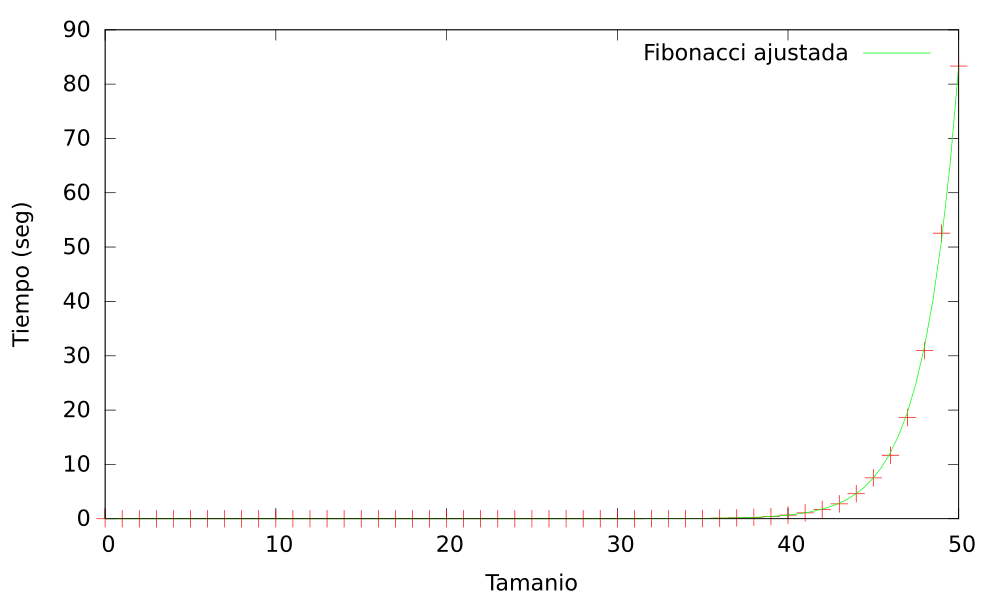
\includegraphics[totalheight=8cm]{img/Fibonacci_ajustada}
		\caption{Ajuste función de Fibonacci}
		\label{fig:Fibonacci_ajustada}
	\end{figure}
	
	\subsection{Algoritmo de Floyd}
	
	
	\begin{longtable}{|c|c|c|}
		\hline
		Constante		& Valor			& Error estándar	\\ \hline
		a0              & 4.5232e-09	& 12.19 \\ \hline
		a1              & 1.64e-06		& 51.27 \\ \hline
		a2              & -0.000541551	& 66.61 \\ \hline
		a3              & 0.0340052		& 121.6 \\ \hline
	\end{longtable}
	
	\begin{figure}[H]
		\centering
		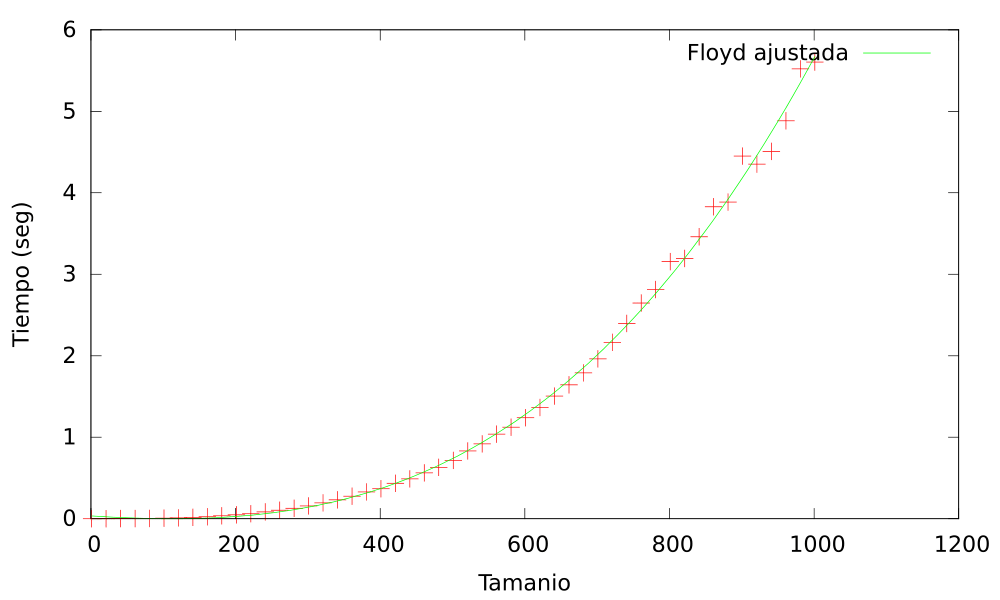
\includegraphics[totalheight=8cm]{img/Floyd_ajustada}
		\caption{Ajuste función de Floyd}
		\label{fig:Floyd_ajustada}
	\end{figure}
	
	Tanto para Floyd como para Fibonacci, el ajuste es de nuevo casi perfecto.
	
	\subsection{Ajustes de tiempos con funciones no correspondientes}
	En este apartado vamos a ajustar nuestros tiempos con funciones teóricas que no se corresponden con su orden de eficiencia.
	\begin{figure}[H]
		\centering
		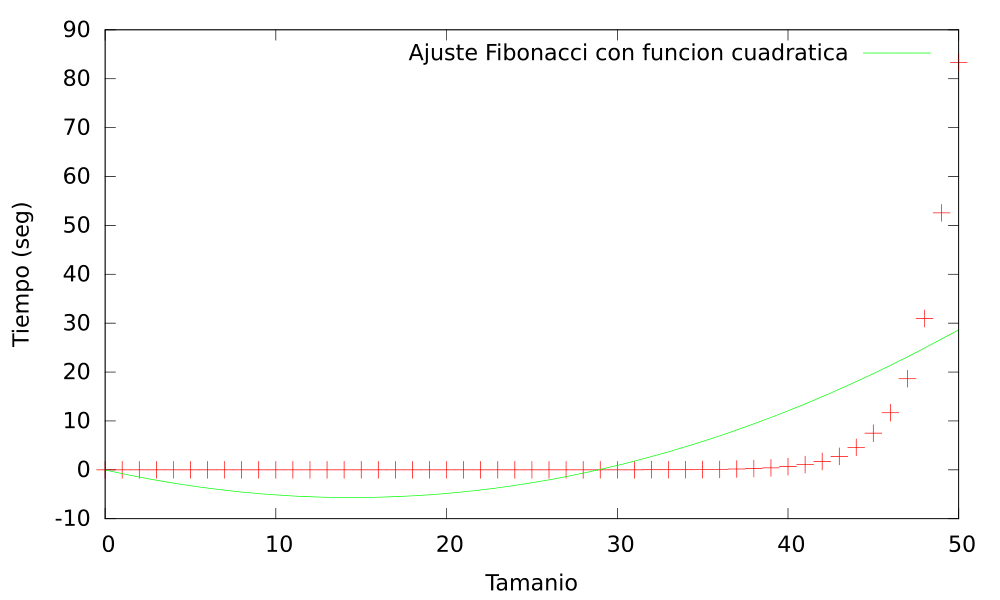
\includegraphics[totalheight=8cm]{img/ajusteFibonacci_cuadratico}
		\caption{Ajuste Fibonacci con función cuadrática}
		\label{fig:ajusteFibonacci_cuadratico}
	\end{figure}
	Aquí vemos que este ajuste es bastante malo. La gráfica cuadrática no se corresponde en prácticamente ningún punto con nuestros tiempos. Cuando empezamos a tener un tamaño de problema superior a 40, Fibonacci se dispara, mientras que la función cuadrática crece mucho más lentamente.
	\begin{figure}[H]
		\centering
		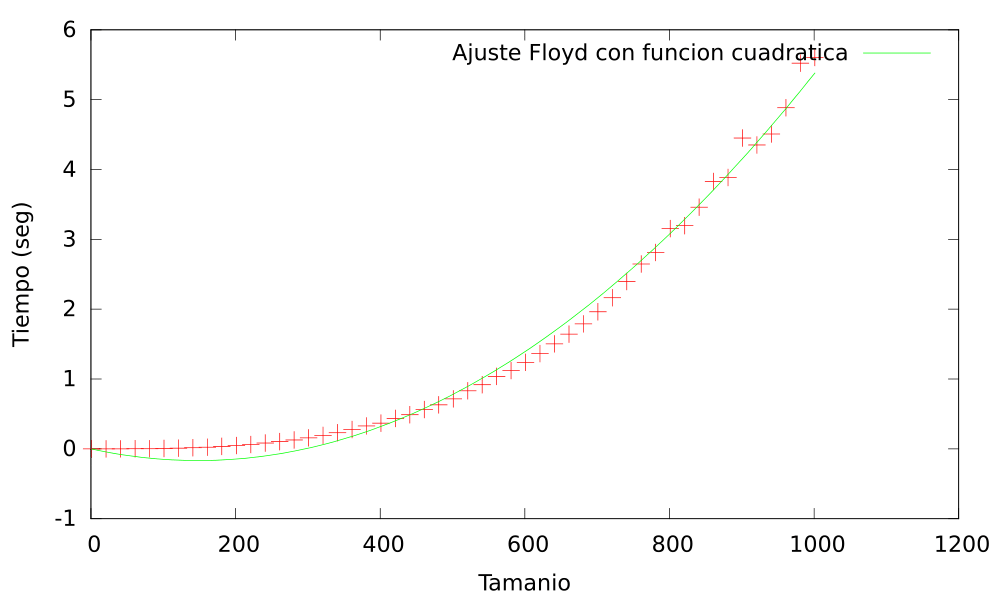
\includegraphics[totalheight=8cm]{img/ajusteFloyd_cuadratico}
		\caption{Ajuste Floyd con función cuadrática}
		\label{fig:ajusteFloyd_cuadratico}
	\end{figure}
	Este ajuste es bastante mejor. Puede ser debido a que el crecimiento de $n^3$ no se dispara hasta que no se alcanzan tamaños más grandes. 
	\begin{figure}[H]
		\centering
		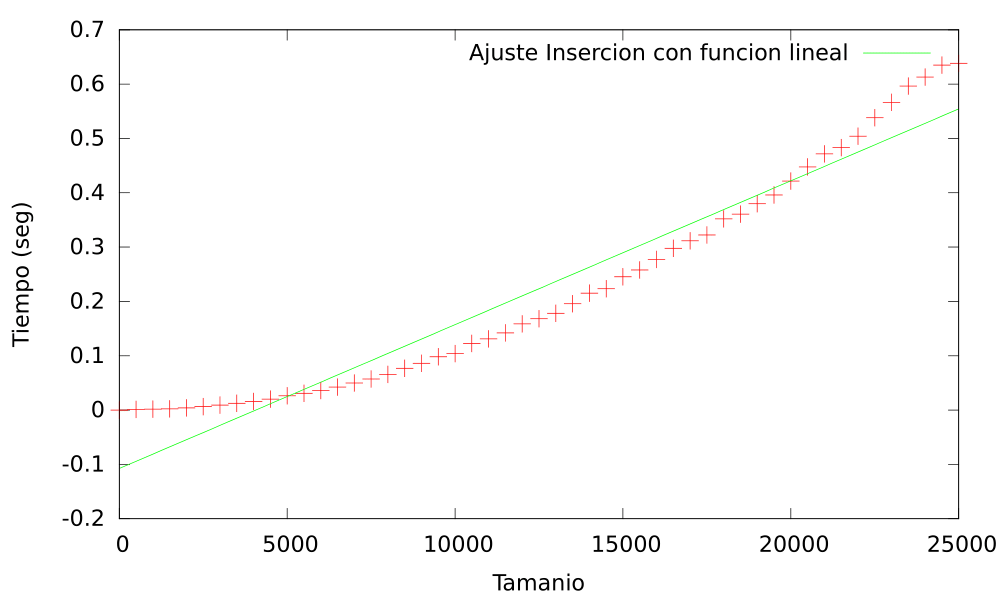
\includegraphics[totalheight=8cm]{img/ajusteInsercion_lineal}
		\caption{Ajuste Inserción con función lineal}
		\label{fig:ajusteInsercion_lineal}
	\end{figure}
	Aquí tenemos otro mal ajuste. Los algoritmos con $O(n^2)$ distan mucho de tener un comportamiento lineal.
	\begin{figure}[H]
		\centering
		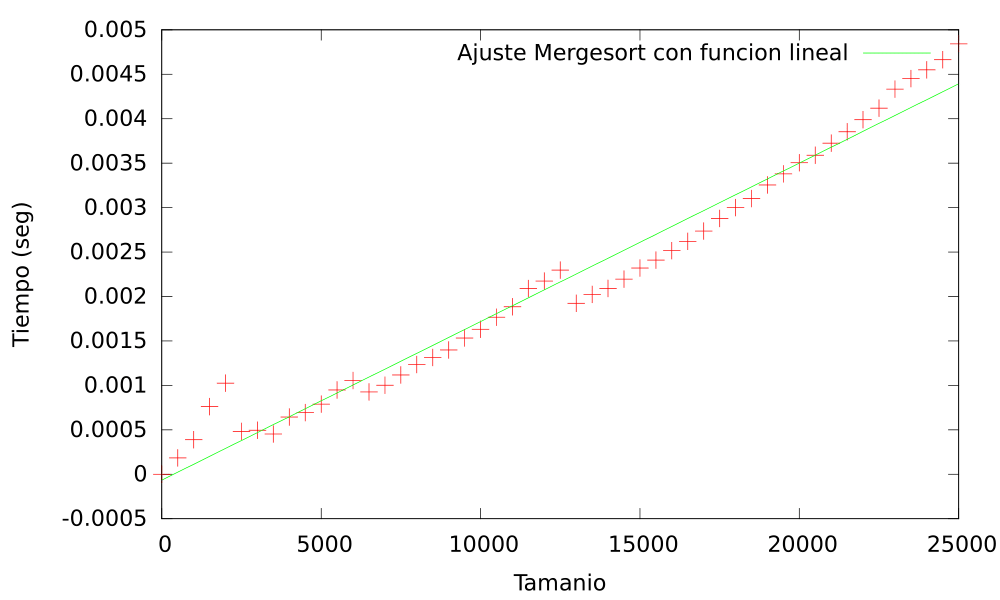
\includegraphics[totalheight=8cm]{img/ajusteMergesort_lineal}
		\caption{Ajuste Mergesort con función lineal}
		\label{fig:ajusteMergesort_lineal}
	\end{figure}
	
	Por último, en esta figura vemos como los algoritmos de ordenación rápida (Mergesort en este caso) sí que pueden comportarse más o menos como un algoritmo lineal aunque sean un poco más lentos.

\subsection{Probando en distintas condiciones}
\subsubsection{Distintos ordenadores}
Hemos probado la misma implementación de un algoritmo en dos ordenadores distintos y así de paso demostrar el principio de invarianza.
\

En la figura \ref{fig:compSeleccion} se muestran los tiempos de ambos ordenadores en la misma gráfica y en la figura \ref{fig:compSeleccion_cociente}, la función cociente entre los tiempos de las dos ejecuciones.
\begin{figure}[H]
	\centering
	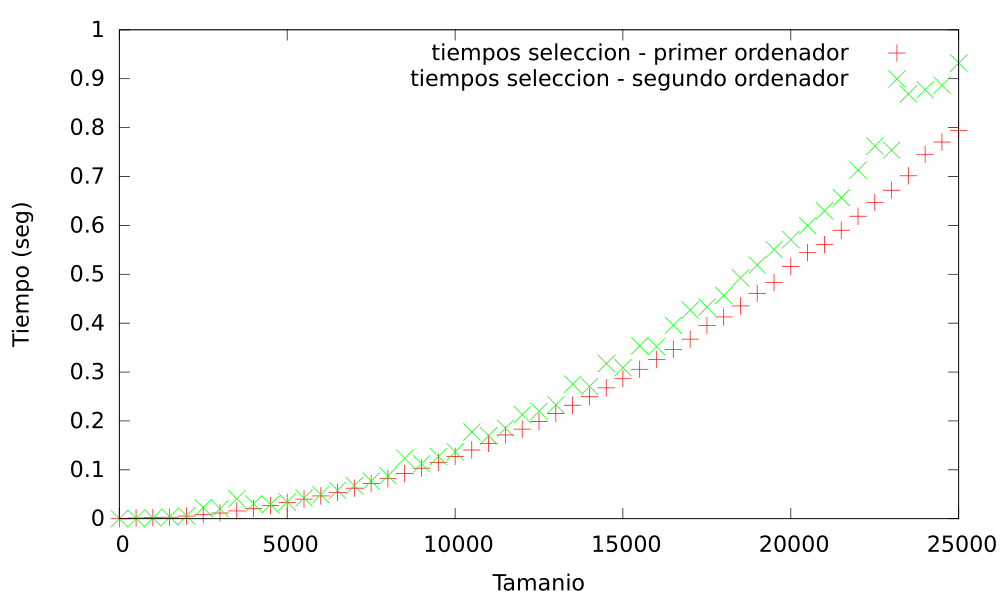
\includegraphics[totalheight=8cm]{img/compSeleccion}
	\caption{Equipos diferentes, tiempos distintos}
	\label{fig:compSeleccion}
\end{figure}
\begin{figure}[H]
	\centering
	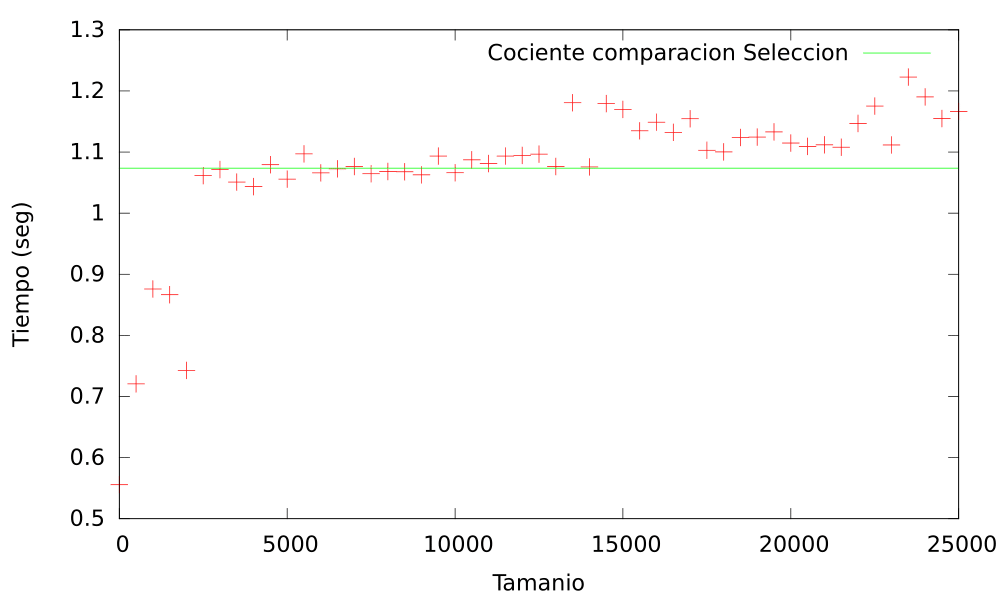
\includegraphics[totalheight=8cm]{img/compSeleccion_cociente}
	\caption{Demostrando el principio de invarianza}
	\label{fig:compSeleccion_cociente}
\end{figure}
\subsubsection{Distintas opciones de compilación}
En este caso hemos probado el algoritmo de Floyd en el mismo equipo, pero compilando con y sin optimización. (Hemos utilizado el \textit{switch} -O3 para la versión optimizada).

\begin{figure}[H]
	\centering
	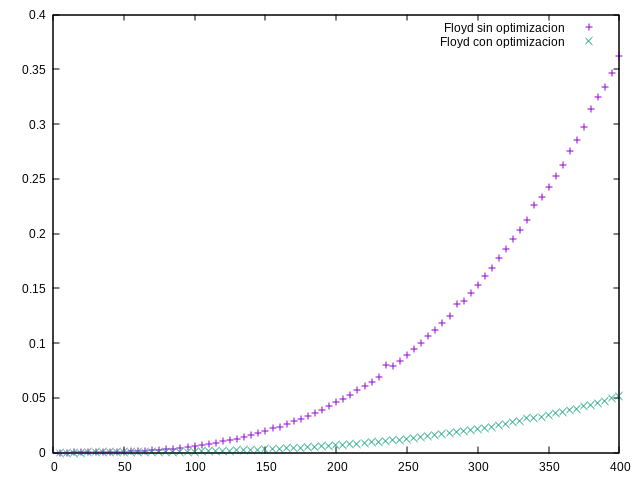
\includegraphics[totalheight=8cm]{img/optimizacion_floyd}
	\caption{Tiempos de ejecución compilando con y sin optimización}
	\label{fig:optimizacion_floyd}
\end{figure}

A pesar de todo, como se muestra en la figura \ref{fig:optimizacion_cociente}, sólo se diferencian en una constante $k \approx 0.141 $.
\begin{figure}[H]
	\centering
	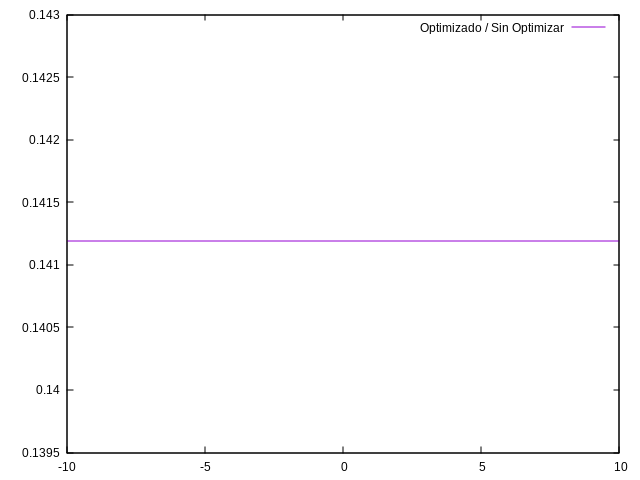
\includegraphics[totalheight=8cm]{img/optimizacion_cociente}
	\caption{El principio de invarianza, esta vez aplicado a las opciones del compilador.}
	\label{fig:optimizacion_cociente}
\end{figure}
\section{Notas}
Los tiempos han sido calculados con {\bf std::chrono} y para las gráficas se ha usado la herramienta {\bf gnuplot}.
\

Para el cálculo de estos tiempos hemos usado un equipo con las siguientes prestaciones:
\begin{itemize}
	\item Arquitectura:                        x86\_64
	\item modo(s) de operación de las CPUs:    32-bit, 64-bit
	\item Orden de los bytes:                  Little Endian
	\item CPU(s):                              8
	\item Lista de la(s) CPU(s) en línea:      0-7
	\item Hilo(s) de procesamiento por núcleo: 2
	\item Núcleo(s) por «socket»:              4
	\item «Socket(s)»                          1
	\item Modo(s) NUMA:                        1
	\item ID de fabricante:                    GenuineIntel
	\item Familia de CPU:                      6
	\item Modelo:                              60
	\item Nombre del modelo:                   Intel(R) Core(TM) i7-4700MQ CPU @ 2.40GHz
	\item Revisión:                            3
	\item CPU MHz:                             1910.940
	\item CPU MHz máx.:                        3400,0000
	\item CPU MHz mín.:                        800,0000
	\item BogoMIPS:                            4788.59
	\item Virtualización:                      VT-x
	\item Caché L1d:                           32K
	\item Caché L1i:                           32K
	\item Caché L2:                            256K
	\item Caché L3:                            6144K
	\item CPU(s) del nodo NUMA 0:              0-7
\end{itemize}
En el apartado 3.6.1 hemos usado un segundo ordenador para comparar, estas son sus características:
\begin{itemize}
	\item Arquitectura:          x86\_64
	\item modo(s) de operación de las CPUs:32-bit, 64-bit
	\item Orden de bytes:        Little Endian
	\item CPU(s):                1
	\item On-line CPU(s) list:   0
	\item Hilo(s) de procesamiento por núcleo:1
	\item Núcleo(s) por «socket»:1
	\item Socket(s):             1
	\item Modo(s) NUMA:          1
	\item ID de fabricante:      GenuineIntel
	\item Familia de CPU:        6
	\item Modelo:                142
	\item Model name:            Intel(R) Core(TM) i7-7500U CPU @ 2.70GHz
	\item Revisión:             9
	\item CPU MHz:               2904.000
	\item BogoMIPS:              5808.00
	\item Fabricante del hipervisor:KVM
	\item Tipo de virtualización:lleno
	\item Caché L1d:            32K
	\item Caché L1i:            32K
	\item Caché L2:             256K
	\item Caché L3:             4096K
	\item NUMA node0 CPU(s):     0
\end{itemize}
\end{document}
